
\subsection{Resumen enunciado}


%\bfseries{\color{red} Enunciado:}

\normalfont

Este TP consiste en realizar un pequeño estudio del movimiento de un ascensor, figura~\figref{fig:fig_elevator}, intentando utilizar valores realistas para los parámetros a fin de obtener las expresiones para la posición, $x_{(t)}$, la velocidad, $v_{(t)}$ y la aceleración, $a_{(t)}$. Luego estas expresiones se utilizarán para aplicar un método numérico de nuestra implementación, Newton-Raphson en este caso.





\subsection{Planteo}

El planteo implica asumir ciertas cosas acerca del ascensor, realizando el análisis para el movimiento ascendente, en particular se debe analizar, la altura de un piso, que asumimos ser igual para todos los pisos, siendo en todos por lo tanto el mismo problema, la masa de la cabina y los pasajeros, el tiempo de viaje máximo (se da a máxima carga), la máxima aceleración, y la máxima velocidad, asumimos también por simplicidad que la fuerza que se imprime a la cabina varía linealmente con el tiempo, esto es planteado así en el enunciado. Todas estos parámetros se obtuvieron de normas locales,\citelink{camaradeascensores}, e internacionales, \citelink{elevatorworld}, y de algunos ejemplos de ascensores residenciales comerciales.



%%\begin{figure}[!h] %htb
\begin{wrapfigure}{r}{0.5 \linewidth}
\begin{center}
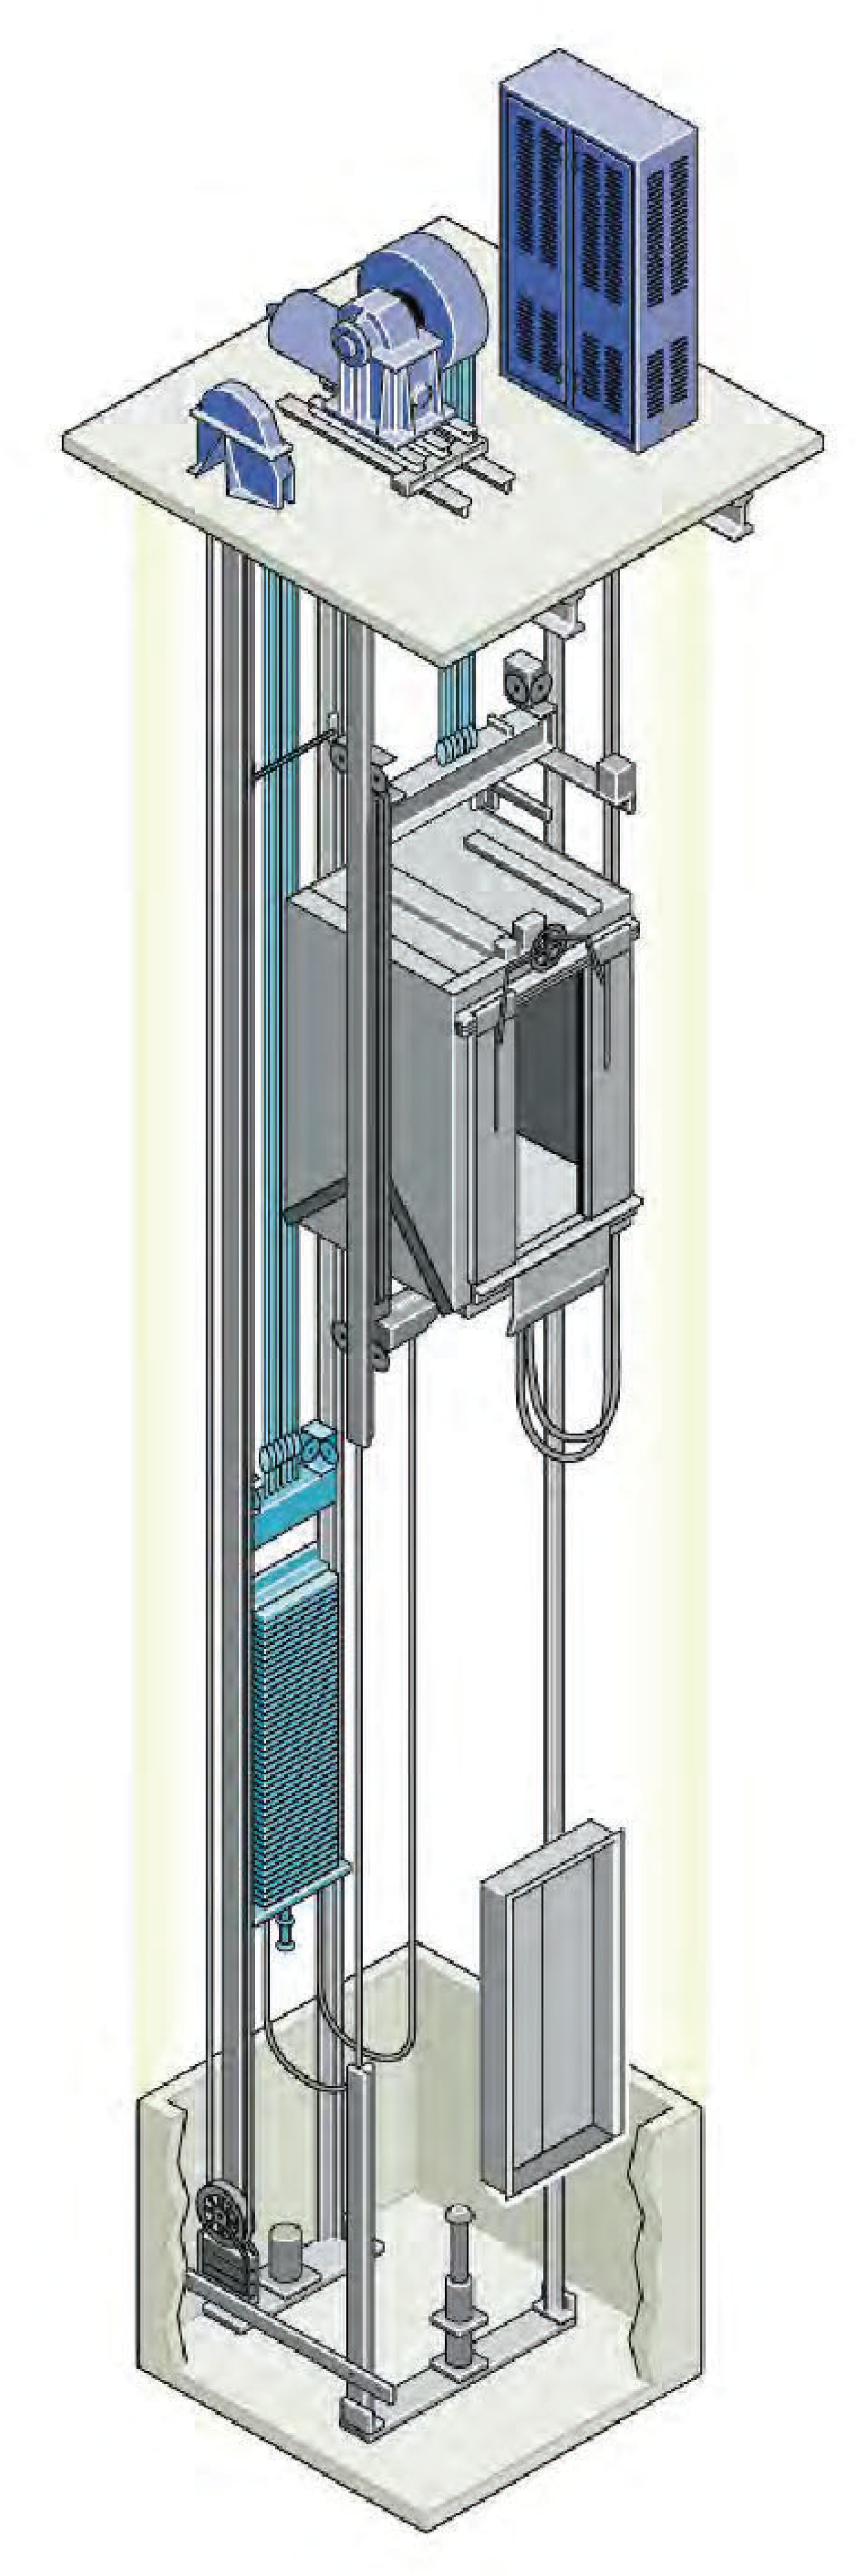
\includegraphics[width=0.35 \linewidth, keepaspectratio=true]{img/diagrams/elevator.png} %% , angle=90 trim={<left> <lower> <right> <upper>}
\caption{\label{fig:fig_elevator} \footnotesize{Ascensor electromecánico.}}
\end{center}
\end{wrapfigure}
%%\end{figure}

En general las normas especifican para la máxima aceleración posible $8 \si[per-mode=symbol]{\meter\per\second\squared}$, la masa de cada persona debe tomarse en promedio como de $75 \si[per-mode=symbol]{\kilogram}$, la masa de la cabina depende del ascensor en cuestión, se tomó un modelo para $12$ personas, con una cabina de masa igual a $450 \si[per-mode=symbol]{\kilogram}$, esto determina la masa máxima de carga en $1350 \si[per-mode=symbol]{\kilogram}$ y la mínima en los $450 \si[per-mode=symbol]{\kilogram}$ de la cabina vacía.


\begin{equation}
x_{(t)} = A \cdot t^{3} + B \cdot t^{2} + C \cdot t + D
\end{equation}

\begin{equation}
v_{(t)} = 3 \cdot A \cdot t^{2} + 2 \cdot B \cdot t + C
\end{equation}

\begin{equation}
a_{(t)} = 6 \cdot A \cdot t + 2 \cdot B \cdot
\end{equation}


\clearpage


\subsection{Resolución}

Para la resolución de la parte de programación del trabajo práctico e implementar los algoritmos pedidos, decidimos usar \textbf{MATLAB}, mayormente por conocerlo previamente y la sencillez con la que se pueden escribir scripts que implementen los algoritmos. A pesar de que la resolución se realizó en \textbf{MATLAB}, se prestó atención a la compatibilidad con \textbf{Octave}, ya que la compatibilidad en los paquetes básicos es alta y con un poco de cuidado y algo de programación condicional se puede lograr que los scripts funcionen en ambos entornos.
Todas las salidas numéricas se guardaron en archivos que luego fueron leídas en \LaTeX\space usando paquetes para el proceso de archivos en formato \textbf{\quotemarks{CSV}}, los mismos permiten redondeo, presentación y hasta algunas operaciones sobre los datos, lo cual facilita el escribir el informe de tal manera de que no deba modificarse al modificar los datos, basta con compilar nuevamente. Las imágenes en forma similar, se guardaron por código desde \textbf{MATLAB} en formato \textbf{\quotemarks{PNG}} y luego se incorporaron desde \LaTeX. Algo a mencionar es que se estimaron lo valores del orden de convergencia y la constante asintótica, para cada uno de los método numéricos implementados, para lograr una buena precisión en las estimaciones se agregó una tolerancia mas a las ya pedidas en el trabajo práctico.


